\documentclass{article}

\usepackage[spanish]{babel}
\usepackage[numbers,sort&compress]{natbib}
\usepackage{graphicx}
\usepackage{url}
\usepackage{amsmath}
\usepackage{hyperref}
\usepackage[top=30mm, bottom=40mm, left=15mm, right=15mm]{geometry}
\usepackage{listings}
\usepackage{subfig}
\usepackage{color}
\usepackage{multirow}
\usepackage[latin1]{inputenc}

\setlength{\parskip}{2mm}
\setlength{\parindent}{0pt}
\definecolor{dkgreen}{rgb}{0,0.6,0}
\definecolor{gray}{rgb}{0.3,0.3,0.3}
\definecolor{orange}{rgb}{0.8,0.4,0}
\definecolor{mostaza}{rgb}{0.9,0.8,0.1}

\lstset{ %
  language=R,                     % the language of the code
  basicstyle=\footnotesize,       % the size of the fonts that are used for the code
  numbers=left,                   % where to put the line-numbers
  numberstyle=\tiny\color{gray},  % the style that is used for the line-numbers
  stepnumber=1,                   % the step between two line-numbers. If it's 1, each line
                                  % will be numbered
  numbersep=5pt,                  % how far the line-numbers are from the code
  backgroundcolor=\color{white},  % choose the background color. You must add \usepackage{color}
  showspaces=false,               % show spaces adding particular underscores
  showstringspaces=false,         % underline spaces within strings
  showtabs=false,                 % show tabs within strings adding particular underscores
  frame=single,                   % adds a frame around the code
  rulecolor=\color{black},        % if not set, the frame-color may be changed on line-breaks within not-black text (e.g. commens (green here))
  tabsize=2,                      % sets default tabsize to 2 spaces
  captionpos=b,                   % sets the caption-position to bottom
  breaklines=true,                % sets automatic line breaking
  breakatwhitespace=false,        % sets if automatic breaks should only happen at whitespace
  title=\lstname,                 % show the filename of files included with \lstinputlisting;
                                  % also try caption instead of title
  keywordstyle=\color{orange},      % keyword style
  commentstyle=\color{dkgreen},   % comment style
  stringstyle=\color{mostaza},      % string literal style
  escapeinside={\%*}{*)},         % if you want to add a comment within your code
  morekeywords={*,...}            % if you want to add more keywords to the set
} 

\author{Marco Antonio Guajardo Vigil  2095}
\title{\textbf{Pr\'actica 6: Sistema multiagente} \\ Simulaci\'on de sistemas}
\date{5 de marzo, 2019}

\begin{document}

\maketitle

\section{Introducci\'on}
Un sistema multiagente es parecido a un aut\'omata celular, hay un conjunto de entidades con estados internos que pueden observar estados de otras entidades y reaccionar cambiando su propio estado. La diferencia es que un sistema multiagente es un concepto m\'as general y permite que estos agentes se muevan y varien su vecindad, entre otras cosas \cite{SatuP6}.

Para esta pr\'actica se implementa un sistema multiagente con una aplicaci\'on en epidemiolog\'ia. Los agentes podr\'an estar en uno de estos tres estados: \textbf{S}usceptibles, \textbf{I}nfectados o \textbf{R}ecuperados, esto se conoce como el modelo \textit{SIR}.
Los par\'ametros son el n\'umero de agentes \textit{n} y la probabilidad de infecci\'on al inicio $p_i$. La infecci\'on produce inmunidad en los recuperados, por lo cual solamente los susceptibles podr\'an ser infectados. La probabilidad de contagio es proporcional a la distancia euclideana entre dos agentes $d(i, j)$ de la siguiente manera:


\begin{center}$p_c = \left \{ \begin{array}{ll}
  0, & \text{ si } d(i, j) \geq r, \\
  \displaystyle\frac{r - d}{r}, & \text{ en otro caso,} \end{array}
  \right.$
\end{center}

donde $r$ es un umbral.

Nuestros agentes tienen coordenadas $x$ y $y$, una direcci\'on y una velocidad (expresadas en t\'erminos de $\Delta x$ y $\Delta y$). Se posicionan los agentes uniformemente al azar en un torus formado por doblar un rect\'angulo de $l \times l$ en dos dimensiones, se observa un ejemplo de un sistema multiagente en la figura \ref{fig:multiagente}.

\begin{figure}[h!]
\centering\includegraphics[width=80mm]{multiagente.png}
\caption{Ejemplo de un sistema multiagente de cincuenta agentes,  tres infectados y cuarenta y siete susceptibles.}
\label{fig:multiagente}
\end{figure}

\section{Objetivo}
Se vacuna con probabilidad $p_v$ a los agentes al momento de crearlos de tal forma que estos inicien en estado \textit{R} y no pueden contagiarse ni propagar la infecci\'on. Se estudia el efecto estad\'istico del valor $p_v$ en el porcentaje m\'aximo de infectados durante la simulaci\'on.

\newpage

\subsection{Implementaci\'on de R}
Para la elaboraci\'on de este experimento, se hace uso de un software libre para computaci\'on estad\'istica y gr\'aficos llamado \citet{R}, el cual nos permite realizar los c\'alculos necesarios para dicho experimento. Con \'el, se pueden controlar los datos estad\'isticos que se ocupan para dar seguimiento con la pr\'actica, se necesita graficarlos para as\'i poder compararlos mejor, ya que se maneja una cantidad de datos considerable y trabajaremos con ellos en forma estad\'istica.

\subsection{Experimentaci\'on}

La simulaci\'on contiene cincuenta agentes representado en la variable \texttt{n}, se crea un \texttt{data.frame()} llamado \texttt{Rvacunas} (en el cual se almacenan los valores de las probabilidades, r\'eplicas, m\'aximo de infectados y porcentaje de esos m\'aximos). La probabilidad de vacunaci\'on se var\'ia en secuencia desde el cero al uno, en pasos de 0.1 y se hacen cincuenta r\'eplicas por cada probabilidad como se muestra en el c\'odigo:

\begin{lstlisting}[language=R]
l <- 1.5 
n <- 50 #numero de agentes
pi <- 0.05 #probabilidad de infeccion al inicio
pr <- 0.02 #probabilidad de recuperacion
v <- l / 30 #velocidad del agente
PV <- seq(0,1,0.1) #probabilidad de vacunacion al inicio
r <- 0.1 #umbral
replicas <- 50
Rvacunas <- data.frame()
\end{lstlisting}

\newpage

Para lograr la variaci\'on se realizan dos \texttt{for()}, uno para las probabilidades de vacunaci\'on y otro para las r\'eplicas, se agrega un \texttt{if()} para vacunar a los agentes de acuerdo a la probabilidad que tengan y un \texttt{while()} que para la simulaci\'on una vez  alcance la mayor cantidad de infectados posible, para eso se toma en cuenta la cantidad de infectados actuales la cual se almacena en la variable \texttt{actual} y se compara con lo que este almacenado en la variable \texttt{mayor} que inicialmente esta en cero, si la variable mayor es menor a actual, mayor toma el valor de actual, as\'i hasta que actual llegue a ser menor que mayor, ya que en ese caso, alcanzo el mayor n\'umero de infectados posibles y se sale del \texttt{while()} con un \texttt{break}, como se muestra en el c\'odigo:

\begin{lstlisting}[language=R]
epidemia <- integer()
mayor <- 0
actual <- 0
for(pv in PV){
  for(rep in 1:replicas){
    if(runif(1) < pv){ #vacunados al inicio con probabilidad pv
        e <- "R"
      } else if(runif(1) < pi){
        e <- "I"
      } else{
        e <- "S"
      }

    while(TRUE){
      ...
      actual <- infectados
      if(mayor < actual){
        mayor <- actual
      } else if(actual < mayor){
        break
      }
    }
    maximo_infectados <- max(epidemia)
    porcentaje <- 100 * maximo_infectados / n
    Rvacunas <- rbind(Rvacunas, c(pv, rep, maximo_infectados, porcentaje))
  }
}
 
\end{lstlisting}

Se crea una gr\'afica con ayuda de la librer\'ia \texttt{ggplot2} \cite{ggplot2} que muestra el porcentaje de infectados m\'aximos que alcanzo la simulaci\'on con tal probabilidad de ser vacunados, esto es para hacer observaciones acerca de lo que llega a influir la vacuna en el sistema:

\begin{lstlisting}[language=R]
tema <- theme(
  panel.background = element_rect(fill = "lightblue", colour = "lightblue", size = 0.5, 
                                   linetype = "solid"),
  panel.grid.major = element_line(size = 0.5, linetype = 'solid', colour = "white"), 
  panel.grid.minor = element_line(size = 0.25, linetype = 'solid',colour = "white")
)
p <- ggplot(Rvacunas, aes(x = Probabilidad, y = Porcentaje, fill = Probabilidad)) + geom_violin()
p <- p + geom_violin(scale = "width", alpha = 0.6) + geom_violin(trim = F) + geom_boxplot(width=0.3, alpha=0.8)
p <- p + labs(x="Probabilidades de vacunaci\u{F3}n", y = "Porcentaje m\u{E1}ximo de infectados") + tema
ggsave("violin.png")
\end{lstlisting}

\newpage

\subsection{Resultados y conclusiones}

\begin{figure}[h!]
\centering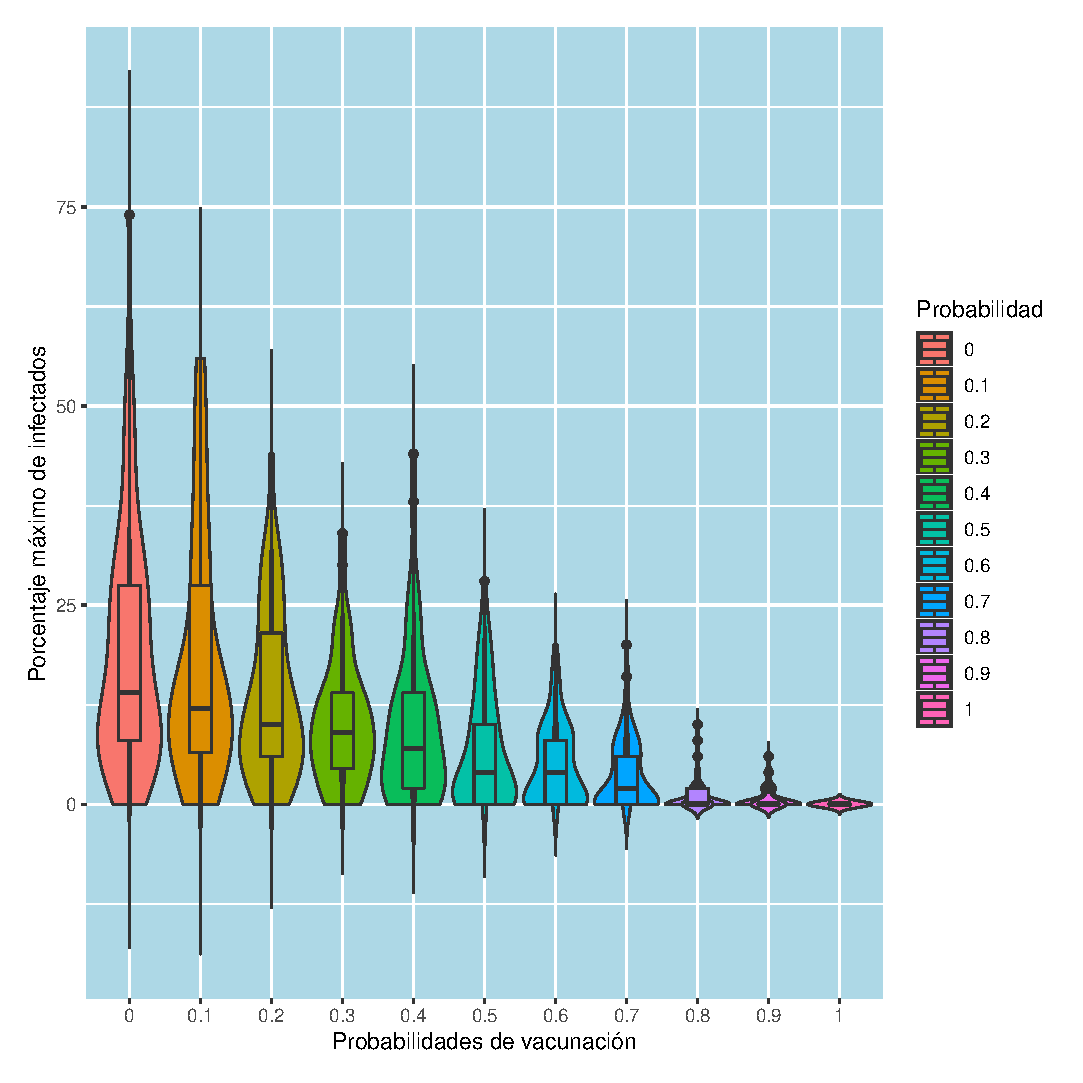
\includegraphics[width=120mm]{ResultadosP6.eps}
\caption{Porcentaje m\'aximo de agentes infectados con relaci\'on a las probabilidades de ser vacunado.}
\label{fig:resultados}
\end{figure}

En la gr\'afica de la figura \ref{fig:resultados} se muestra que las probabilidades que m\'as afectan en la epidemia son $p_v > 0,2$ aproximadamente, estas probabilidades empiezan a bajar el m\'aximo de infectados considerablemente, por lo tanto, s\'i afecta la probabilidad en el crecimiento de agentes infectados. Esto se comprueba con un test probabil\'istico de \textit{Kruskal-Wallis}, el cual fue realizado con ayuda del paquete \texttt{nortest}, con el cual obtenemos un valor $p$ que nos garantiza si afectan esas probabilidades.

\begin{lstlisting}[language=R]
kruskal.test(Rvacunas$Porcentaje~Rvacunas$Probabilidad)
\end{lstlisting}

Por lo general, un nivel de significaci\'on (indicado como $\alpha $ o alfa) de 0,05 funciona bien. Este nivel indica que no hay una diferencia real \'o afectaci\'on considerable. El valor de $p \leq  \alpha $, muestra que las diferencias entre algunas de las medianas son estad\'isticamente significativas \cite{kruskal}.

Si el valor de $p$ es menor o igual que el nivel de significaci\'on, podemos concluir que las probabilidades si afectaron en los infectados de la epidemia.
Con la prueba se obtuvo $p-value < 2.2 e-16$, esto es menor al nivel de significaci\'on, por lo tanto, las probabilidades si afectan considerablemente en la epidemia, el n\'umero de infectados baja exponencialmente conforme la probabilidad de vacunacion es m\'as alta.

\section{Reto 1}

El objetivo de este primer reto es cambiar los patrones de movimiento de modo que no tengan una trayectoria fija utilizando el modelo de \textit{punto medio aletorio} (En ingl\'es: random waypoint model).
Cada agente tiene una posici\'on meta $(x,y)$ hacia la cual se mueve con cierta velocidad $v$; al alcanzar o superar su meta, se elige una nueva meta uniformemente al azar. 

La velocidad de cada agente es una constante, normalmente distribuido sobre la poblaci\'on de agentes. Se examina si surgen cambios en el efecto de $p_v$  con esta modificaci\'on.

\subsection{Experimentaci\'on}

Se modifica el c\'odigo de manera que los agentes cambien sus patrones de movimiento, estableciendo nuevas metas para $(x,y)$, se asigna una probabilidad de cambio de meta $p_c$ para que el movimiento del agente cambie cada cierto tiempo, esto se realiza sumando a la posici\'on siguiente (meta) un n\'umero aleatorio dado en rangos de velocidad: $-v < m < v$, en donde $m$ puede tomar valores establecidos entre ese rango:

\begin{lstlisting}[language=R]
pc <- 0.1
if(reto1){
  if(runif(1) < pc){ #probabilidad de nueva meta
    a$x <- a$x + runif(1,-v,v)
    a$y <- a$y + runif(1,-v,v)
  } else{
    a$x <- a$x + a$dx
    a$y <- a$y + a$dy
  }
} else{
  a$x <- a$x + a$dx
  a$y <- a$y + a$dy
}
\end{lstlisting}

Ya que se obtienen variaciones en los movimientos de los agentes, se procede a realizar de nuevo el experimento anterior, vacunando inicialmente a los agentes con probabilidad $p_v$, siendo esta probabilidad la secuencia desde el cero al uno, en pasos de 0.1. Se realizan cincuenta r\'eplicas para mejores estimaciones.

\subsection{Resultados y conclusiones}

Se realizo la prueba probabil\'istica de \textit{Kruskal-Wallis} para comparar si se presentan cambios en los efectos de las probabilidades. El valor de significaci\'on fue el mismo a como cuando cada uno de los agentes ten\'ian el mismo patr\'on de movimiento durante la duraci\'on de la epidemia, lo cual significa que las fijaciones de nuevas metas no afectaron al valor significativo de las probabilidades de vacunaci\'on. 

Con respecto a la gr\'afica de la figura \ref{fig:resultadosR1} se observa que el cambio de patrones afecta a la cantidad m\'axima de infectados siendo de un 55\%, anteriormente de un 75\%,  por lo tanto, tener nuevos patrones de movimiento hacen que la epidemia sea m\'as dif\'icil de propagarse.

\newpage

\begin{figure}[h!]
\centering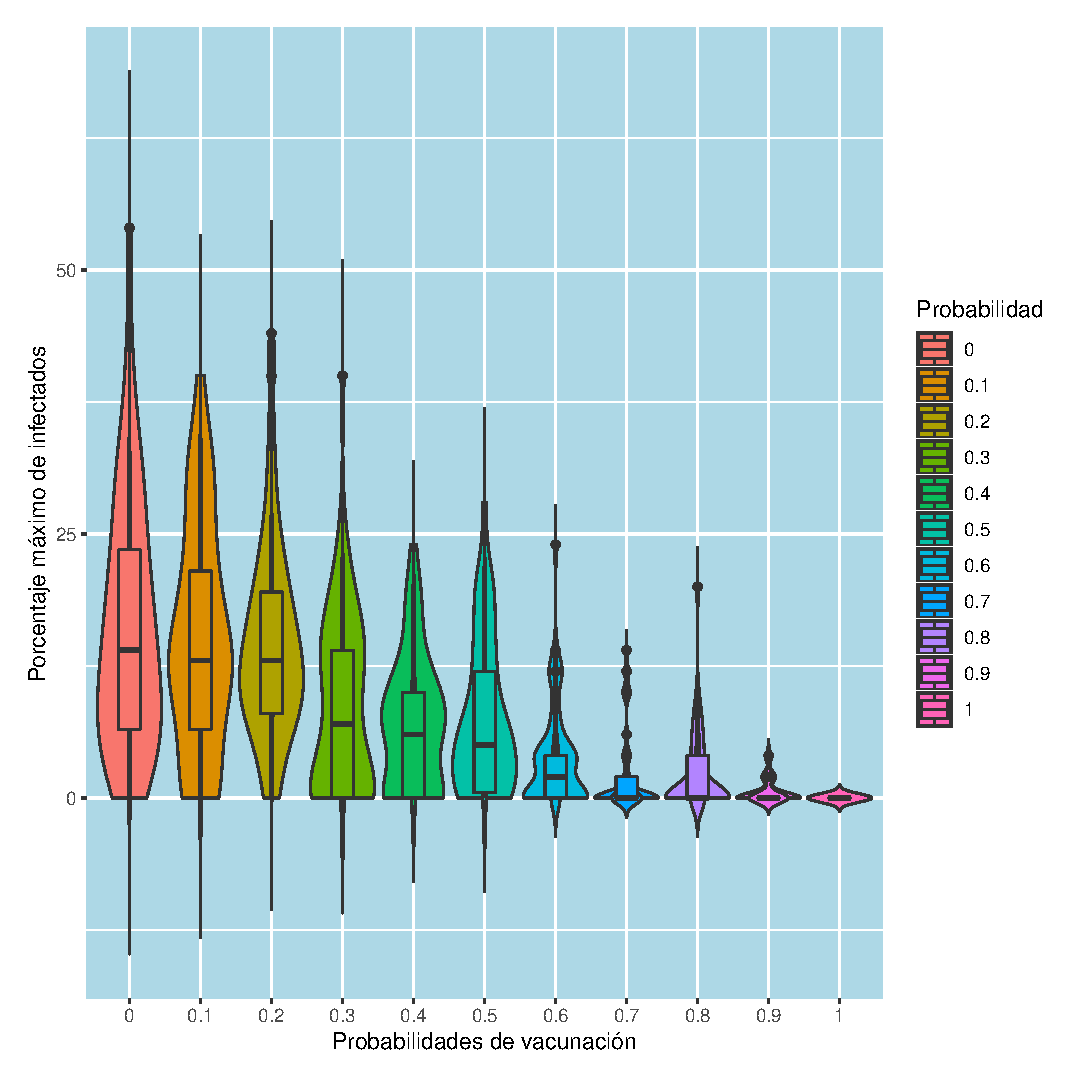
\includegraphics[width=120mm]{ResultadosP6R1.eps}
\caption{Porcentaje m\'aximo de agentes infectados con relaci\'on a las probabilidades de ser vacunado respecto al efecto punto medio aleatorio.}
\label{fig:resultadosR1}
\end{figure}

\section{Reto 2}

El objetivo de este segundo reto es asignar amistades a los agentes, de manera que si se encuentran en una distancia euclideana no mayor a $r_a$ de un amigo suyo, disminuyen su velocidad a la mitad por $k_a$ iteraciones (para saludar a su amigo).

Se examina nuevamente si surgieron cambios en el efecto de $p_v$ por esta modificaci\'on, se eligen los valores con las siguientes condiciones: $0 < r_a < 1$,  $k_a  >  1$ y $0 < p_a < 1$.

\newpage

\subsection{Experimentaci\'on}

La asignaci\'on de amistades se logra con la probabilidad $p_a = 0.6$, esto se realiza al comienzo junto a la asignaci\'on de estados de los agentes. Para que un agente detecte que un agente amigo esta cercas de \'el con una distancia euclideana menor a la de su amigo $r_a = 0.8$, se realiza un \texttt{if()} que permita evaluar esa condici\'on y tambi\'en se debe de cumplir que exista una amistad entre esos dos agentes, cuando esto suceda, se reducira la velocidad de ambos a la mitad hasta que termine el n\'umero de iteraciones o pasos $k_a$. Todo esto se ve representado en el siguiente c\'odigo:

\begin{lstlisting}[language=R]
ka <- 6 
ra <- 0.8 #distancia de amigo
pa <- 0.6 #probabilidad de amistad

agentes <- data.frame(x = double(), y = double(), dx = double(), dy = double(), estado  = character(), amigo = NULL)

#asignar amistad
if(runif(1) < pa){
  amistad <- TRUE
} else{
  amistad <- FALSE
}

agentes <- rbind(agentes, data.frame(x = runif(1, 0, l), y = runif(1, 0, l),
                                           dx = runif(1, -v, v), dy = runif(1, -v, v),
                                           estado = e, amigo = amistad))

for(pv in PV){
  for(rep in 1:replicas){
    ...
    pasos <- ka
    #bajar la velocidad a la mitad cuando se encuentre a un amigo
     if(d < ra && a1$amigo == a2$amigo){
       if(pasos == ka){
         dx <- dx / 2
         dy <- dy / 2
         pasos <- pasos - 1
         #print("baja")
       } else if(pasos > 0){
          pasos <- pasos - 1
       } else{ #regresa a su velocidad normal
          dx <- dx * 2
          dy <- dy * 2
          #print("normaliza")
           pasos <- ka
        }
      }
   }
}
\end{lstlisting}

Se procede a realizar la simulaci\'on variando la probabilidad de las vacunas al comienzo y se grafican los datos obtenidos para llegar a una conclusi\'on y definir si las amistades entre agentes llegan a tener alg\'un afecto significativo \'o no en la proporci\'on de los m\'aximos infectados con relaci\'on a la probabilidad de vacunaci\'on.

\subsection{Resultados y conclusiones}

Estos resultados, visibles en la figura \ref{fig:resultadosR2}, muestran un porcentaje de infectados mayor a los anteriores debido al momento en que los agentes bajan su velocidad tienen m\'as riesgo de encontrarse con alg\'un agente infectado, adem\'as de que el agente amigo puede estar tambi\'en infectado. Esto solo afecta al porcentaje de infectados pero sigue el mismo comportamiento dependiendo de la probabilidad de vacunaci\'on, mientras m\'as alta sea, menos infectados hay. La gr\'afica ahora se asemeja m\'as a la de una exponencial.

En la figura \ref{fig:comparacion} se observa mejor como llego a ser el porcentaje de infectados en los tres casos.

\begin{figure}[h!]
\centering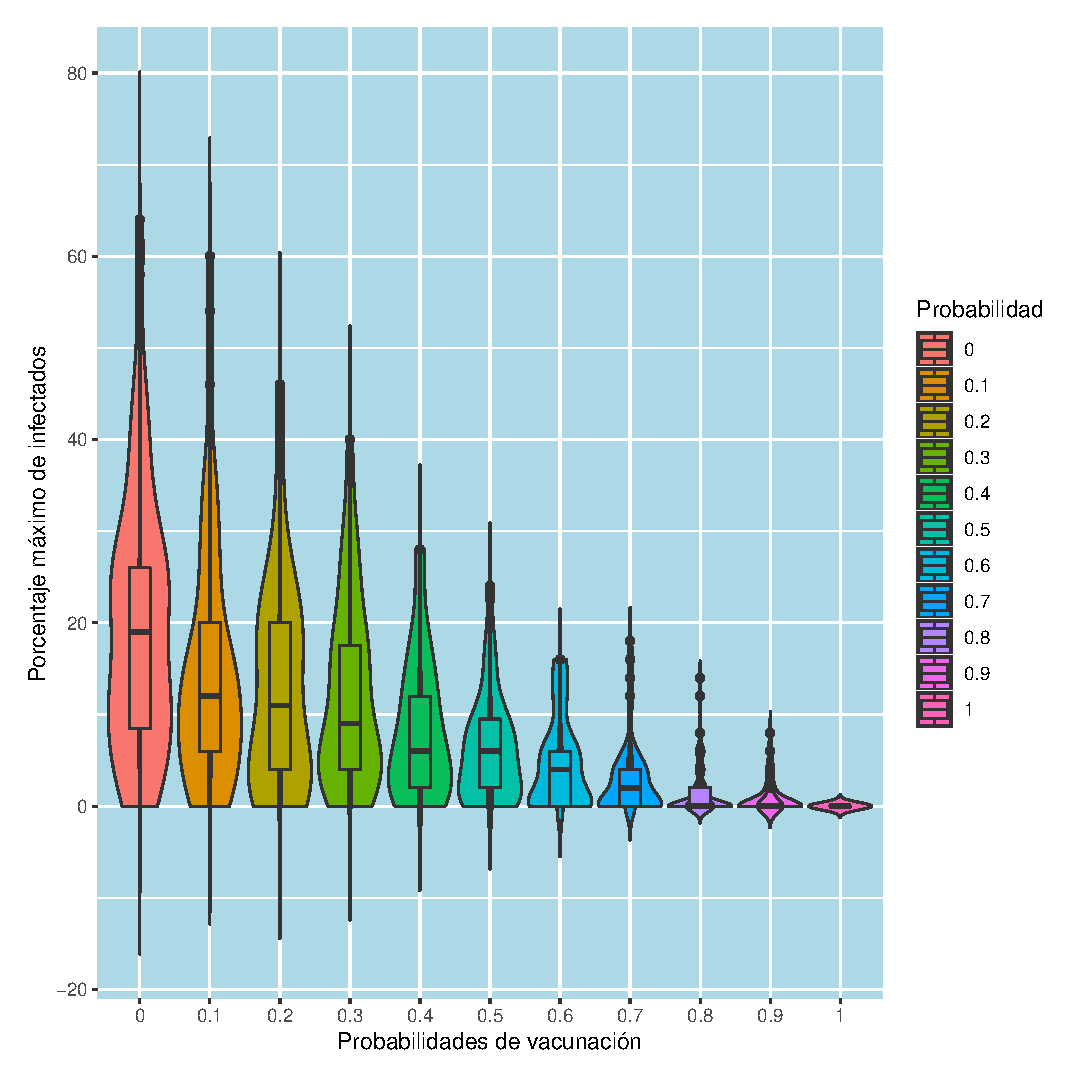
\includegraphics[width=105mm]{ResultadosP6R2.eps}
\caption{Porcentaje m\'aximo de agentes infectados con relaci\'on a las probabilidades de ser vacunado respecto al efecto de las amistades que tienen los agentes.}
\label{fig:resultadosR2}
\end{figure}

\begin{figure}[h!]
 \centering
  \subfloat[Probabilidades de vacunaci\'on con relaci\'on al mayor porcentaje de infectados.]{
   \label{fig:p6}
    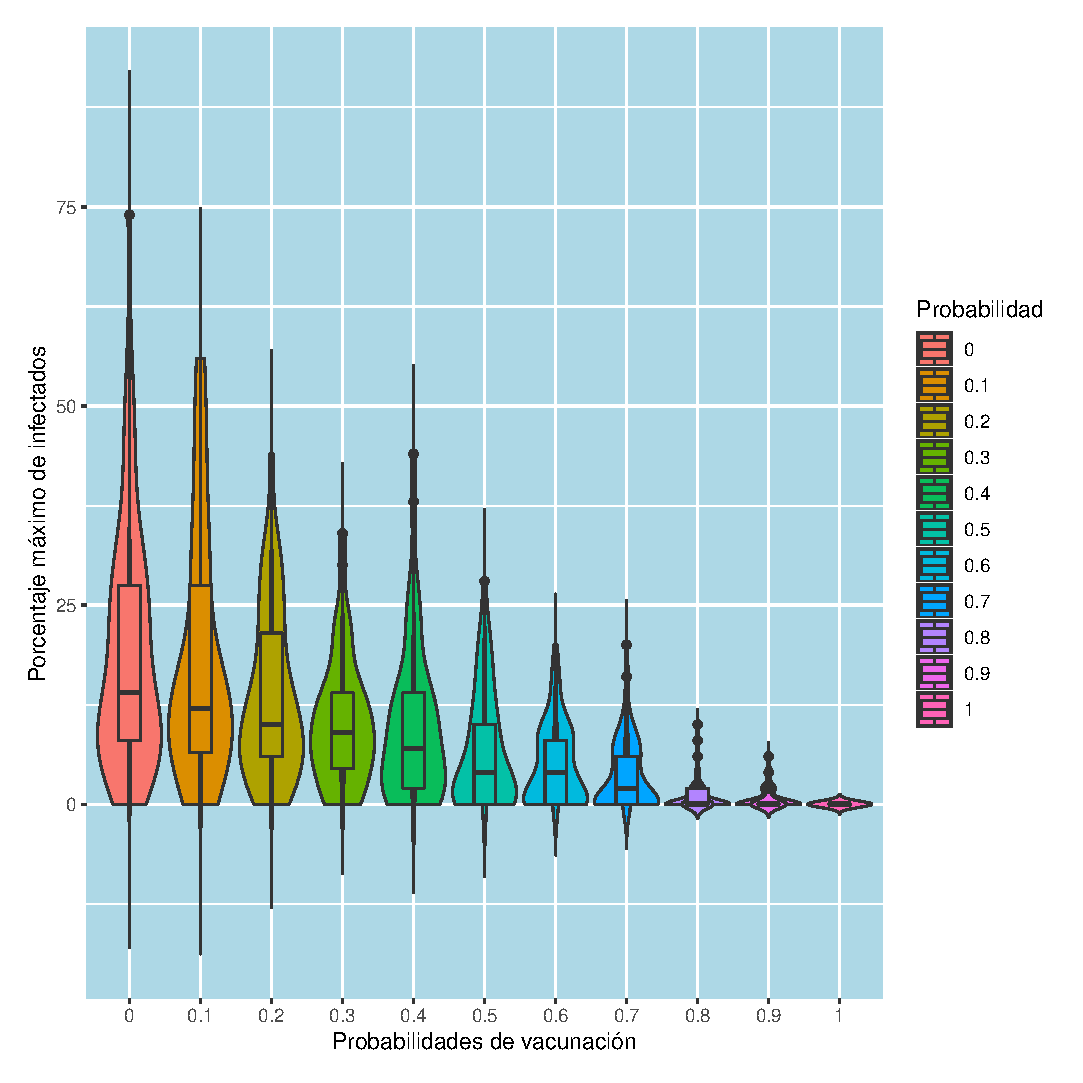
\includegraphics[width=60mm]{ResultadosP6.eps}}
 \subfloat[Efecto de punto medio aleatorio.]{
   \label{fig:p6r1}
    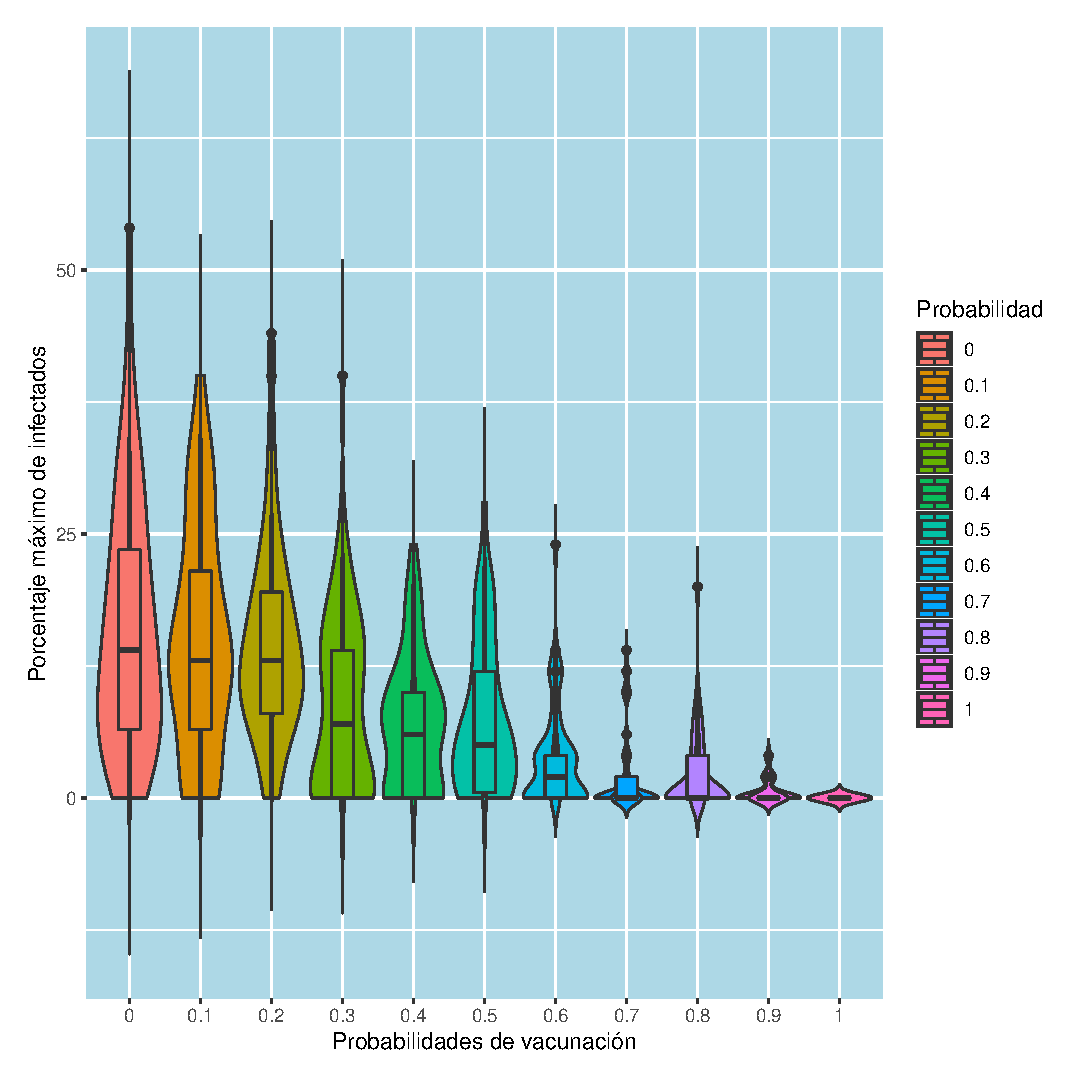
\includegraphics[width=60mm]{ResultadosP6R1.eps}}
  \subfloat[Efecto de agentes con amistades.]{
   \label{fig:p6r2}
    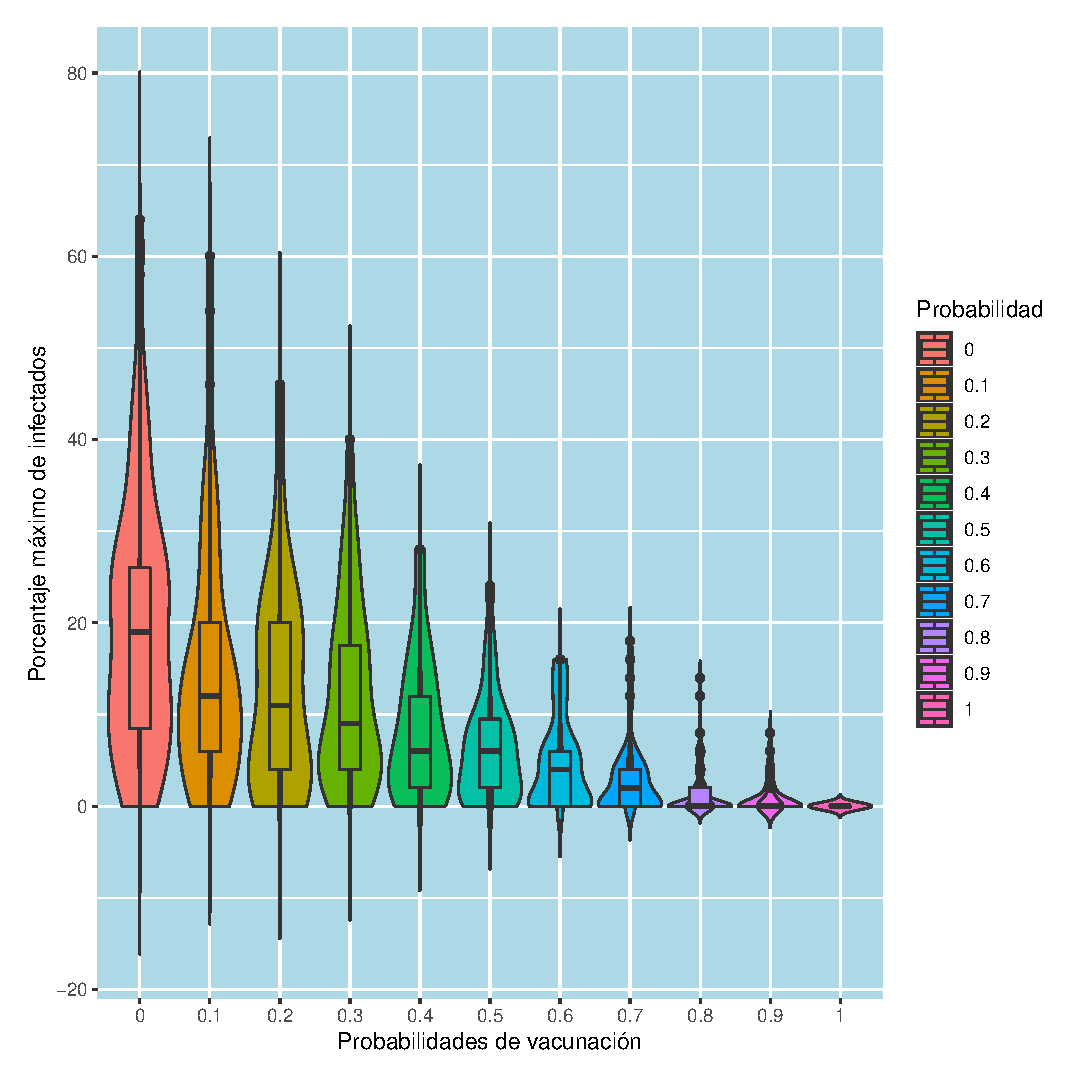
\includegraphics[width=60mm]{ResultadosP6R2.eps}}
 \caption{Comparaci\'on de los efectos realizados en cada reto de acuerdo a la tarea principal.}
 \label{fig:comparacion}
\end{figure}


\newpage

\bibliographystyle{plainnat}
\bibliography{Bibliografias}
\end{document}